\documentclass[border=4pt]{standalone}
\usepackage[utf8]{luainputenc}
\usepackage[T1]{fontenc}
\usepackage[dvipsnames]{xcolor}
\usepackage{cmbright}

\definecolor{blue1tab20}{RGB}{31,119,180} 
\definecolor{blue2tab20}{RGB}{174,199,232} 
\definecolor{orange1tab20}{RGB}{255,127,14} 
\definecolor{orange2tab20}{RGB}{255,187,120} 
\definecolor{green1tab20}{RGB}{44,160,44} 
\definecolor{green2tab20}{RGB}{152,223,138} 
\definecolor{red1tab20}{RGB}{214,39,40} 
\definecolor{red2tab20}{RGB}{255,152,150}
\definecolor{violet1tab20}{RGB}{148,103,189} 
\definecolor{violet2tab20}{RGB}{197,176,213}
\definecolor{brown1tab20}{RGB}{140,86,75} 
\definecolor{brown2tab20}{RGB}{196,156,148} 
\definecolor{pink1tab20}{RGB}{227,119,194} 
\definecolor{pink2tab20}{RGB}{247,182,210} 
\definecolor{gray1tab20}{RGB}{127,127,127} 
\definecolor{gray2tab20}{RGB}{199,199,199} 
\definecolor{olive1tab20}{RGB}{188,189,34} 
\definecolor{olive2tab20}{RGB}{219,219,141} 
\definecolor{lightblue1tab20}{RGB}{23,190,207} 
\definecolor{lightblye2tab20}{RGB}{158,218,229}
\definecolor{greenlink}{HTML}{228B22}

\definecolor{greenbright}{HTML}{4AE44A}
\definecolor{greendark}{HTML}{00B000}
\definecolor{bluebright}{HTML}{4FD8FA}
\definecolor{bluedark}{HTML}{0080FF}
\definecolor{redbright}{HTML}{FF6349}
\definecolor{reddark}{HTML}{C10534}
\definecolor{violetbright}{HTML}{E346E3}
\definecolor{violetdark}{HTML}{800080}

\definecolor{greenline}{HTML}{229222}
\definecolor{blueline}{HTML}{245A90}
\definecolor{redline}{HTML}{91223E}
\definecolor{violetline}{HTML}{871F87}

\definecolor{grayno}{HTML}{BFBFBF}
% color list: https://en.wikibooks.org/wiki/LaTeX/Colors

\usepackage{pgfplots}
\pgfplotsset{compat=1.16}
\usepgfplotslibrary{fillbetween}
\usetikzlibrary{calc}


% https://tex.stackexchange.com/questions/238022/how-to-specify-the-starting-point-of-a-horizontal-bar-in-latex

\begin{document}

\pgfplotsset{scaled y ticks=false}
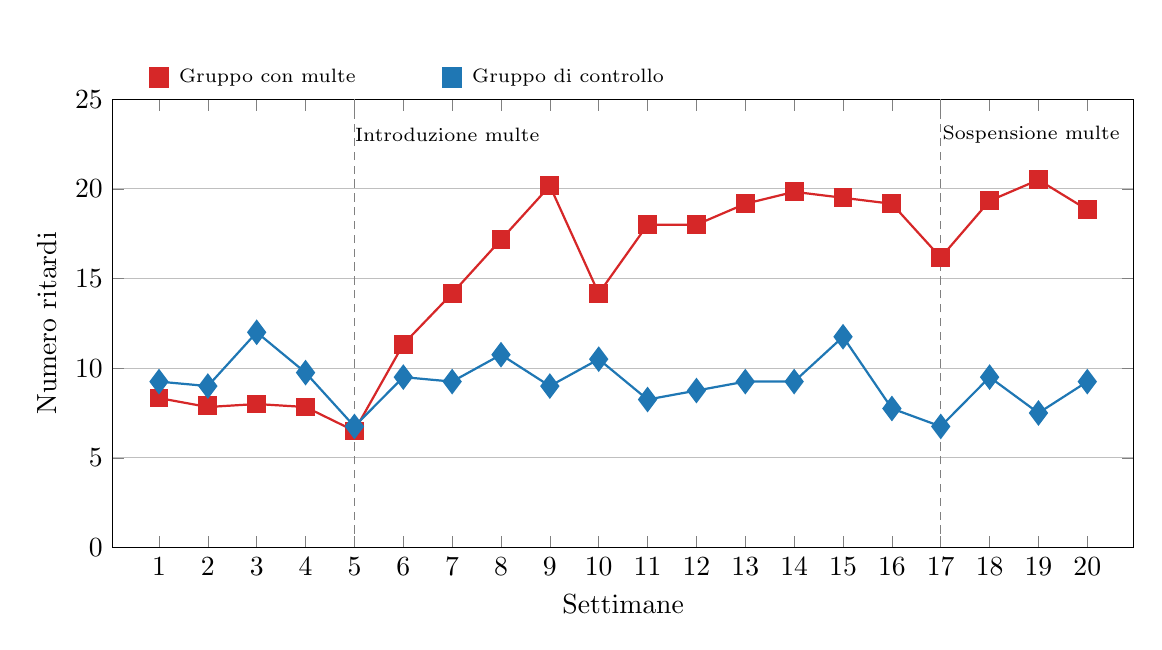
\begin{tikzpicture}

\tikzstyle{sqblue} = [rectangle, fill opacity=1, text opacity=1, minimum height=7pt, minimum width=7pt, align=center, fill=blue1tab20, draw=blue1tab20]
\tikzstyle{sqred} = [rectangle, fill opacity=1, text opacity=1, minimum height=7pt, minimum width=7pt, align=center, fill=red1tab20, draw=red1tab20]


\begin{axis}[
enlarge x limits=0.05,
%enlarge y limits=0.1,
width=414, % default = 240pt
height=207pt, % default = 207pt
xmin = 1,
xmax = 20,
xtick = {1,2,...,20},
ymin = 0,
ymax = 25,
ytick = {0,5,...,25},
ylabel style={align=center, text width=207pt},
ylabel={Numero ritardi},
xlabel={Settimane},
%ylabel near ticks,
ymajorgrids,
%extra x ticks = {1, 2, 3, 4, 5, 6, 7, 8, 9, 10},
xticklabel style   = {align=center,rotate=0}, %align=right
%extra x tick labels = {{Nov01}, {Nov02}, {Mar03}, {Jun03}},
%extra y tick labels = {0, 0.25, 0.50, 0.75, 1},
%axis on top,
clip mode = individual
]

\draw[densely dashed,gray] (5,0)--(5,25);
\draw[densely dashed,gray] (17,0)--(17,25);

\node[align=left] at (6.9,23) {\scriptsize Introduzione multe};
\node[align=left] at (18.85,23) {\scriptsize Sospensione multe};

\addplot[xbar, only marks, mark = square*, mark size = 3pt, red1tab20, thick]  coordinates {(1,8.333)};
\addplot[xbar, only marks, mark = square*, mark size = 3pt, red1tab20, thick]  coordinates {(2,7.933)};
\addplot[xbar, only marks, mark = square*, mark size = 3pt, red1tab20, thick]  coordinates {(3,8)};
\addplot[xbar, only marks, mark = square*, mark size = 3pt, red1tab20, thick]  coordinates {(4,7.833)};
\addplot[xbar, only marks, mark = square*, mark size = 3pt, red1tab20, thick]  coordinates {(5,6.5)};
\addplot[xbar, only marks, mark = square*, mark size = 3pt, red1tab20, thick]  coordinates {(6,11.333)};
\addplot[xbar, only marks, mark = square*, mark size = 3pt, red1tab20, thick]  coordinates {(7,14.166)};
\addplot[xbar, only marks, mark = square*, mark size = 3pt, red1tab20, thick]  coordinates {(8,17.166)};
\addplot[xbar, only marks, mark = square*, mark size = 3pt, red1tab20, thick]  coordinates {(9,20.166)};
\addplot[xbar, only marks, mark = square*, mark size = 3pt, red1tab20, thick]  coordinates {(10,14.166)};
\addplot[xbar, only marks, mark = square*, mark size = 3pt, red1tab20, thick]  coordinates {(11,18)};
\addplot[xbar, only marks, mark = square*, mark size = 3pt, red1tab20, thick]  coordinates {(12,18)};
\addplot[xbar, only marks, mark = square*, mark size = 3pt, red1tab20, thick]  coordinates {(13,19.166)};
\addplot[xbar, only marks, mark = square*, mark size = 3pt, red1tab20, thick]  coordinates {(14,19.833)};
\addplot[xbar, only marks, mark = square*, mark size = 3pt, red1tab20, thick]  coordinates {(15,19.5)};
\addplot[xbar, only marks, mark = square*, mark size = 3pt, red1tab20, thick]  coordinates {(16,19.166)};
\addplot[xbar, only marks, mark = square*, mark size = 3pt, red1tab20, thick]  coordinates {(17,16.166)};
\addplot[xbar, only marks, mark = square*, mark size = 3pt, red1tab20, thick]  coordinates {(18,19.333)};
\addplot[xbar, only marks, mark = square*, mark size = 3pt, red1tab20, thick]  coordinates {(19,20.5)};
\addplot[xbar, only marks, mark = square*, mark size = 3pt, red1tab20, thick]  coordinates {(20,18.833)};

\draw[red1tab20,thick] (1,8.333)--(2,7.833)--(3,8)--(4,7.833)--(5,6.5)--(6,11.333)--(7,14.166)--(8,17.166)--(9,20.166)--(10,14.166)--(11,18)--(12,18)--(13,19.166)--(14,19.833)--(15,19.5)--(16,19.166)--(17,16.166)--(18,19.333)--(19,20.5)--(20,18.833);

\addplot[xbar, only marks, mark =diamond*, mark size = 4pt,  blue1tab20, thick]  coordinates {(1,9.25)};
\addplot[xbar, only marks, mark =diamond*, mark size = 4pt,  blue1tab20, thick]  coordinates {(2,9)};
\addplot[xbar, only marks, mark =diamond*, mark size = 4pt,  blue1tab20, thick]  coordinates {(3,12)};
\addplot[xbar, only marks, mark =diamond*, mark size = 4pt,  blue1tab20, thick]  coordinates {(4,9.75)};
\addplot[xbar, only marks, mark =diamond*, mark size = 4pt,  blue1tab20, thick]  coordinates {(5,6.75)};
\addplot[xbar, only marks, mark =diamond*, mark size = 4pt,  blue1tab20, thick]  coordinates {(6,9.5)};
\addplot[xbar, only marks, mark =diamond*, mark size = 4pt,  blue1tab20, thick]  coordinates {(7,9.25)};
\addplot[xbar, only marks, mark =diamond*, mark size = 4pt,  blue1tab20, thick]  coordinates {(8,10.75)};
\addplot[xbar, only marks, mark =diamond*, mark size = 4pt,  blue1tab20, thick]  coordinates {(9,9)};
\addplot[xbar, only marks, mark =diamond*, mark size = 4pt,  blue1tab20, thick]  coordinates {(10,10.5)};
\addplot[xbar, only marks, mark =diamond*, mark size = 4pt,  blue1tab20, thick]  coordinates {(11,8.25)};
\addplot[xbar, only marks, mark =diamond*, mark size = 4pt,  blue1tab20, thick]  coordinates {(12,8.75)};
\addplot[xbar, only marks, mark =diamond*, mark size = 4pt,  blue1tab20, thick]  coordinates {(13,9.25)};
\addplot[xbar, only marks, mark =diamond*, mark size = 4pt,  blue1tab20, thick]  coordinates {(14,9.25)};
\addplot[xbar, only marks, mark =diamond*, mark size = 4pt,  blue1tab20, thick]  coordinates {(15,11.75)};
\addplot[xbar, only marks, mark =diamond*, mark size = 4pt,  blue1tab20, thick]  coordinates {(16,7.75)};
\addplot[xbar, only marks, mark =diamond*, mark size = 4pt,  blue1tab20, thick]  coordinates {(17,6.75)};
\addplot[xbar, only marks, mark =diamond*, mark size = 4pt,  blue1tab20, thick]  coordinates {(18,9.5)};
\addplot[xbar, only marks, mark =diamond*, mark size = 4pt,  blue1tab20, thick]  coordinates {(19,7.5)};
\addplot[xbar, only marks, mark =diamond*, mark size = 4pt,  blue1tab20, thick]  coordinates {(20,9.25)};

\draw[blue1tab20,thick] (1,9.25)--(2,9)--(3,12)--(4,9.75)--(5,6.75)--(6,9.5)--(7,9.25)--(8,10.75)--(9,9)--(10,10.5)--(11,8.25)--(12,8.75)--(13,9.25)--(14,9.25)--(15,11.75)--(16,7.75)--(17,6.75)--(18,9.5)--(19,7.5)--(20,9.25);

\node[sqblue] (sqblue) at (7,26.2) {};
\node[right] at (sqblue.east) {\scriptsize Gruppo di controllo};

\node[sqred] (sqred) at (1,26.2) {};
\node[right] at (sqred.east) {\scriptsize Gruppo con multe};

%\node (prob) at (6,17) {\scriptsize Technical problem};
%\draw[->] (prob) -- (6,6.7);

\end{axis}

\end{tikzpicture}
\end{document}







